\documentclass[a4paper, 12pt]{article}

\usepackage[left = 1cm,
            right = 1cm,
            top = 1cm,
            bottom = 1.5cm,
            footskip = 0cm]{geometry}
\usepackage{graphicx} % Required for inserting images
\usepackage{wrapfig}
\usepackage{listings}
\usepackage{xcolor}

\linespread{0.9}
\setlength{\parskip}{0pt}

\definecolor{codebackground}{rgb}{0.95,0.95,0.92} % Couleur de fond du code
\definecolor{codepurple}{rgb}{0.58, 0, 0.82}
\definecolor{codegreen}{rgb}{0, 0.6, 0}

\lstdefinestyle{mystyle}{
    language=C++,
    basicstyle=\scriptsize\ttfamily,
    frame=single,
    rulecolor=\color{black},
    backgroundcolor=\color{codebackground},
    commentstyle=\color{codegreen},
    keywordstyle=\color{blue},
    numberstyle=\tiny\color{codepurple},
    stringstyle=\color{red},
    lineskip={-1.5pt}
}

\lstset{style=mystyle}

\title{\textbf{Rapport pour le projet de INFOF202}}
\author{
    Ransy Lenny
    \and
    Lejeune Lucas
    }
\date{Janvier 2024}
\renewcommand*\contentsname{Table des matières}

\begin{document}
\setlength{\parindent}{0em}

\maketitle

Ce rapport vise à documenter le projet "Frogger" que nous avons réalisé. 
Nous traiterons les tâches que nous avons réalisées et comment nous les avons réalisées. 
Pour cela, nous parlerons des classes que nous avons codées pour faire ce projet, 
comment elles sont réparties dans le code et comment elles interagissent entre elles. 
Nous justifierons également comment nous avons utilisé le modèle de conception MVC dans 
la partie jeu. \\

Nous avons réalisé les tâches principales et toutes les tâches additionnelles, 
sauf la tâche de l'éditeur de niveau. 


\section{Structure des fichiers: Utilisation du MVC}
% Parler de l'orga des fichiers
\begin{wrapfigure}{r}{3cm}
    \centering
    \vspace{-0.8cm}
    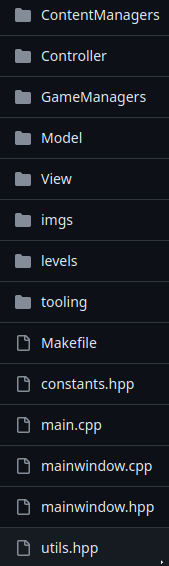
\includegraphics[width=2.5cm]{Images/folders.png}
\end{wrapfigure}

La structure des fichiers peut se diviser en plusieurs parties : les fichiers du jeu, 
ceux des menus, les mains et les images du jeu. \\

- Le dossier \texttt{ContentManagers} contient tous les fichiers de code en rapport 
avec la gestion des menus du jeu. \\
- Les dossiers \texttt{Controller}, \texttt{Model} et \texttt{View} 
contiennent le code permettant de faire tourner le jeu 
(la partie plateau, qui n'inclut pas le menu).
Cette disposition met en évidence l'utilisation du MVC. 
Tout le code de ces fichiers est utilisé dans les fichiers de \texttt{GameManagers} 
pour avoir un jeu fonctionnel. \\
- Le dossier \texttt{levels} contient les données des niveaux sauvegardés en fichiers 
\texttt{.csv}, et les scores obtenus sur ceux-ci. \\
- Le dossier  \texttt{imgs} contient les images utilisées dans le programme. \\
- Le dossier \texttt{tooling} contient tous les outils construits grâce aux outils 
venant de la librairie FLTK qui sont surtout utilisés dans la partie 
\texttt{View} et \texttt{ContentManagers}. \\
- Le fichiers \texttt{constants.hpp} contient toutes les constantes utilisées dans le projet,
comme par exemple la taille des bouttons dans le menu. \\
- Enfin, les fichiers \texttt{main.cpp} et \texttt{mainwindow.hpp} s'occupent 
d'assembler toutes les classes et fonctions pour obtenir l'application Frogger 
au complet. 

\section{Réalisation de la base du jeu (Tâches de base)}
% On parle du tout début juste avec les roadlanes
Bien sûr, pour cette tâche, 
la première chose à faire a été de faire un support pour utiliser tous nos objets.
C'est là que les fichiers \texttt{main.cpp} et \texttt{MainWindow.hpp} rentrent en jeu. 
Les classes et méthodes utilisées dans les classes suivantes seront bien sûr 
abordées dans la suite. 

\begin{lstlisting}
int main(int argc, char *argv[]) {
    std::srand(static_cast<unsigned>(time(nullptr)));
    auto c = std::make_shared<ContentManager>(nullptr);
    auto ws = std::make_unique<WelcomeScreen>(c);
    c->changeContents(std::move(ws));
    MainWindow window(c);
    window.show(argc, argv);
    return Fl::run();
}
\end{lstlisting}

\pagebreak

\begin{lstlisting}
class MainWindow : public Fl_Window {
    private:
        std::shared_ptr<ContentManager> contents;
    public:
        MainWindow(std::shared_ptr<ContentManager> contents);
        void draw() override;
        int handle(int event) override;
        static void Timer_CB(void *userdata);
};
\end{lstlisting}

\subsection{Modèle}

Il nous faut maintenant un modèle fonctionnel. 
Le but est d'abord de créer un plateau de jeu.
Tout ceci se passe dans le dossier \texttt{Model}.

Les rangées sont des objets de classe \texttt{Lane}, 
classe qui est définie dans le fichier \texttt{lanes.hpp}.

\begin{lstlisting}
class Lane {
    private:
        const unsigned int id_num;
    public:
        Lane(const unsigned int id_num);
        unsigned int getId() const;
        virtual void diveUpdate() {}
        virtual ~Lane() {}
};  
\end{lstlisting}

La classe \texttt{BoardModel} représente le plateau de jeu.

\begin{lstlisting}
class BoardModel {
private:
    std::shared_ptr<FinishLane> the_finish_lane;
    std::vector<std::shared_ptr<Lane>> lanes {};
    unsigned time = 0;
public:
    BoardModel(std::vector<std::shared_ptr<Lane>> lanes);
    void updateTurtles(std::shared_ptr<Lane> lane);
    void update(); // moves the objects on the board
    bool gameWon();
    bool isOutOfBoard(Frog& frog);
    bool frogOnLily(Frog& frog);
    void addLane(std::shared_ptr<Lane> lane);
    std::vector<std::shared_ptr<Lane>> getLanes();
    bool anyCollision(Frog& frog);
    void handleCollision(Frog& frog);
    ~BoardModel() {}
    unsigned getTime() const  { return time; }
};
\end{lstlisting}

Pour avoir différents types de rangées, 
il suffit de définir ces types grâce à de l'héritage sur la classe \texttt{Lane}. 
Nous définissons alors dans le fichier \texttt{lane.hpp} 
les classes \texttt{FinnishLane} (nous en parlerons dans le chapitre \ref{lilies}), 
\texttt{SafeLane} et \texttt{RoadLane}, qui représentent respectivement 
la ligne d'arrivée, 
les rangées sans obstacle
et les routes de voitures.

\begin{lstlisting}
class SafeLane: public Lane {
    public:
        SafeLane(const unsigned int id);
        ~SafeLane() {}
};
\end{lstlisting}

\begin{lstlisting}
class MovingObjectLane: public Lane {
    protected:
        std::vector<std::shared_ptr<MovingObject>> mv;
        int lane_speed;
    public:
        MovingObjectLane(const unsigned int id, int lane_speed=0);
        bool frogCollide(Frog& frog);
        std::vector<std::shared_ptr<MovingObject>> getMovingObjects();
        virtual void handleAfterCollision(Frog& frog) = 0;
        virtual bool waterLane() const = 0 ;
        virtual ~MovingObjectLane() {}
};
\end{lstlisting}

\pagebreak

\begin{lstlisting}
class RoadLane: public MovingObjectLane {
    public:
        RoadLane(const unsigned int id_num
                , const unsigned int& car_by_pack
                , const unsigned int& space_between_cars
                , const unsigned& space_between_packs
                , const int& first_car_placement
                , const unsigned int& size_car
                , const int& speed=1);
        bool waterLane() const override { return 0; }
        void handleAfterCollision(Frog& frog) override;
        std::vector<std::shared_ptr<Car>> getCars() const;
         ~RoadLane() {}
};
\end{lstlisting}

Nous voulons d'abord définir ce qu'est une voiture, 
ceci se passe dans le fichier \texttt{movingobjects.hpp}. 

\begin{lstlisting}
class MovingObject {
    protected:
        const int speed;
        int x;
        const unsigned int size;
        const unsigned int lane_id;
    public:
        MovingObject(const int speed, int x, const unsigned int size, const unsigned lane_id);
        void move();
        unsigned getSize() const;
        unsigned getId() const;
        // returns the x coordinate of the center of the object
        int getCenterX() const;
        std::tuple<int, int> getBoundaries() const;
        int getX() const;
        // returns true if this element collides with the frog
        virtual bool collide(Frog& frog) = 0;
        int getSpeed() const;
      
        // Methods regarding diving turtles
        virtual void dive() {}
        virtual void undive() {}
        virtual bool isDiving() const;
        virtual ~MovingObject() {}
};
\end{lstlisting}

\begin{lstlisting}
class Car: public MovingObject {
public:
    Car(int speed, unsigned int head, const unsigned int size, const unsigned lane_id);
    bool collide(Frog& frog) final override;
    ~Car() {}
};
\end{lstlisting}

Parlons maintenant de la grenouille. 
Elle sera définie par un objet de classe \texttt{Frog}, 
classe qui est définie dans le fichier \texttt{frog.hpp}.

\begin{lstlisting}
class Frog {
    private:
        // Frog Position and Direction (important for display)
        unsigned int lane_number;
        int x;
        FrogDirection direction = FrogDirection::North;
        int lives;
        std::shared_ptr<Score> score;
    public:
        Frog(unsigned int lane_number, int x, std::shared_ptr<Score> score);

        // Standard getters
        unsigned int getLane() const ;
        int getX() const;
        int getLives() const;
        FrogDirection getDirection() const;

        // Methods in charge of moving the frog (interacting with the controller)
        void goUp();
        void goDown();
        void goLeft();
        void goRight();

        // Moves the frog in a given direction (helpful when frog is sitting on logs)
        void go(int speed);
        // Returns false only if the frog is outside
        bool inBoard();

        // Methods in charge of life and death of the frog
        void resetPos();
        bool alive();
        void kill();
        void inWaterLilies();

        ~Frog(){}
};
\end{lstlisting}

\subsection{Controlleur}

Les contrôles de la grenouille se passent dans la classe \texttt{Controller} 
qui se trouve dans le fichier \texttt{controller.hpp} qui est contenu dans 
le dossier \texttt{Controller}.
La classe \texttt{Frog} possède déjà des méthodes permettant de changer sa position 
sur le plateau, il faut alors juste les utiliser lorsque nous appuyons sur une touche. 
La méthode \texttt{processKey} sert à gérer ces actions. 
Les contrôles se font avec les touches ZQSD comme pour beaucoup de jeux. 

\begin{lstlisting}
class Controller {
    private:
        std::shared_ptr<Frog> f;
        std::map<char, bool> is_pressed;
        unsigned int count = 0;
    public:
        Controller(std::shared_ptr<Frog> f);
        void decrement();
        void processKey(char& c);
        void updatePressedKeys(const char&& c);
        void resetPressedKeys();
        ~Controller() {}
};
\end{lstlisting}

\subsection{Vue}

Tout ce dont nous allons parler dans ce sous-chapitre se passe dans le dossier \texttt{View}. 
Pour résumer, pour presque chaque classe de la partie modèle, 
il y a une classe de la partie vue qui s'occupe de l'affichage des objets de cette classe.
L'intérêt de ces classes est de pouvoir utiliser la méthode \texttt{draw} pour afficher les
objets sur le plateau. 

\underline{Dans movingobjectview.hpp:}

\begin{lstlisting}
class MovingObjectView {
    protected:
        std::shared_ptr<MovingObject> mv;
        std::unique_ptr<RectangleDrawer> object_drawer;
    public:
        MovingObjectView(std::shared_ptr<MovingObject> mv);
        virtual void draw();
        std::shared_ptr<MovingObject> getMovin();
        virtual ~MovingObjectView() {}
};
\end{lstlisting}

\begin{lstlisting}
class CarView: public MovingObjectView {
    public:
        CarView(std::shared_ptr<Car> c);
        ~CarView() {}
};
\end{lstlisting}

\underline{Dans laneview.hpp:}

\begin{lstlisting}
class LaneView {
    protected:
        std::shared_ptr<Lane> lane;
        LaneDrawer ld;
    public:
        LaneView(std::shared_ptr<Lane> lane);
        virtual void draw() = 0;
        static std::shared_ptr<LaneView> makeView(std::shared_ptr<Lane> l);
        virtual ~LaneView() {}
};
\end{lstlisting}

\begin{lstlisting}
class SafeLaneView: public LaneView {
    public:
        SafeLaneView(std::shared_ptr<SafeLane> sfl);
        void draw() final override;
        ~SafeLaneView() {}
};
\end{lstlisting}

\begin{lstlisting}
class RoadLaneView: public LaneView {
    private:
        std::vector<std::shared_ptr<CarView>> cv;
    public:
        RoadLaneView(std::shared_ptr<RoadLane> rl);
        void draw() final;
        ~RoadLaneView() {}
};
\end{lstlisting}

Nous parlerons de l'affichage de la grenouille dans les chapitres 
\ref{lives} et \ref{frogview}. \\

\pagebreak

\underline{Dans boardview.hpp:}

\begin{lstlisting}
class BoardView {
    private:
        std::vector<std::shared_ptr<LaneView>> lanes;
        std::shared_ptr<BoardModel> b;
    public:
        BoardView(std::vector<std::shared_ptr<LaneView>> lanes,
                    std::shared_ptr<BoardModel> b);
        void draw();
        std::vector<std::shared_ptr<LaneView>> getLaneList();
        ~BoardView() {}
};
\end{lstlisting}

Les outils utilisés pour afficher les éléments du jeu avec FLTK se trouvent tous 
dans le dossier \texttt{tooling}. 
Comme ceux-ci ne sont que des outils et n'ont pas d'impact sur le fonctionnement 
du jeu en lui-même, 
nous n'en parlerons pas dans ce rapport.

\subsection{Assemblage pour faire un jeu fonctionnel}

Il nous faut maintenant assembler le tout pour faire un plateau fonctionnel. 
Ceci se fait dans le dossier \texttt{GameManagers}, et plus particulièrement 
dans le fichier \texttt{gameloop.hpp}. 

\begin{lstlisting}
class GameLoop {
    private:
        std::shared_ptr<BoardModel> bm;
        std::shared_ptr<BoardView> bv;
        std::shared_ptr<FrogView> fv;
        std::shared_ptr<Frog> frog;
        std::shared_ptr<Score> score;
        std::shared_ptr<ScoreView> sv;
        std::shared_ptr<Controller> c;
        std::unique_ptr<ScoreSaver> ssv;
        std::shared_ptr<Score> best_score;
        std::unique_ptr<ScoreView> bs_show;
        const FullScreenJPEGImage lost_screen {"imgs/lose.jpeg" };
        const FullScreenJPEGImage won_screen {"imgs/won.jpeg"};

    public:
        GameLoop(unsigned int lvl);
        void update();
        std::shared_ptr<BoardModel> getModel();
        std::shared_ptr<BoardView> getView();
        std::shared_ptr<FrogView> getFrog();
        ~GameLoop() {}
};
\end{lstlisting}


\section{Réalisation des tâches additionnelles}

Maintenant que les tâches principales sont réalisées et que nous avons une bonne base, 
nous pouvons implémenter les fonctionnalités supplémentaires. 

\subsection{Rangées d'eau, buches et tortues} \label{turtle_class}

\underline{\textbf{Modèle:}} 
Dans le fichier \texttt{movingobjects.hpp}, nous implémentons les tortues et les buches. 

\begin{lstlisting}
class Turtle: public MovingObject {
    private:
        bool diving;
    public:
        Turtle(int speed, const unsigned int head, const unsigned int size
                , const unsigned lane_id);
        void dive() final override;
        void undive() final override;
        bool isDiving() const final override;
        bool collide(Frog& frog) final override;
        ~Turtle() {}
};
\end{lstlisting}

\begin{lstlisting}
class Log: public MovingObject {
    public:
        Log(int speed, unsigned int head, const unsigned int size,
            const unsigned lane_id);
        bool collide(Frog& frog) final override;
        ~Log() {}
};
\end{lstlisting} 

\pagebreak

Dans le fichier \texttt{lane.hpp}, nous implémentons deux nouvelles classes héritantes de \texttt{MovingObjectLane}.

\begin{lstlisting}
class LogLane: public MovingObjectLane {
    public:
        LogLane(const unsigned int id_num, const unsigned int& log_by_pack,
                const unsigned int& space_between_logs,
                const unsigned& space_between_packs,
                const int& first_log_placement,
                const unsigned int& size_log, const int& speed=0);
        bool waterLane() const override { return 1; }
        void handleAfterCollision(Frog& frog) override;
        std::vector<std::shared_ptr<Log>> getLogs() const;
        ~LogLane() {}
};
\end{lstlisting}

\begin{lstlisting}
class TurtleLane: public MovingObjectLane {
    unsigned int turtle_by_pack;
    unsigned int diving_pack_id;
    bool is_diving = true;
    unsigned int diving_time;   // In frames
    unsigned int undiving_time;
    unsigned int diving_count = 0;
    public:
        TurtleLane(const unsigned int id_num
                   , const unsigned int& turtle_by_pack
                   , const unsigned int& space_between_turtles
                   , const unsigned& space_between_packs
                   , const int& first_turtle_placement
                   , const unsigned int& size_turtle
                   , const int& speed=1
                   , const unsigned int diving_pack_id = 0
                   , const unsigned int diving_time = 180
                   , const unsigned int undiving_time = 180);
        std::vector<std::shared_ptr<Turtle>> getTurtles() const;
        void handleAfterCollision(Frog& frog) override;
        bool waterLane() const override { return 1; }
        void packDive();
        void packUndive();
        void diveUpdate() final override;
        ~TurtleLane() {}
};
\end{lstlisting}

\underline{\textbf{Vue:}} \\
Les implémentations gérant la vue de ces deux nouvelles rangées est similaire que pour celle 
des rangées de voitures.
\begin{lstlisting}
class LogView: public MovingObjectView {
    public:
        LogView(std::shared_ptr<Log> l);
        ~LogView() {}
};
\end{lstlisting}

\begin{lstlisting}
class TurtleView: public MovingObjectView {
    public:
        TurtleView(std::shared_ptr<Turtle> t);
        void draw() final override;
        ~TurtleView() {}
};
\end{lstlisting}

\subsection{Nénuphars} \label{lilies}

Dans le fichier \texttt{waterlilies.hpp}, 
nous définissons une nouvelle classe \texttt{WaterLilies} qui va représenter les nénuphars. 

\begin{lstlisting}
class WaterLilies {
    private:
        int x;
        bool visited=false;
    public:
        WaterLilies(int x);
        int getX();
        bool collide(Frog& frog);
        bool hasBeenVisited();
        void visit();
        ~WaterLilies() {}
};
\end{lstlisting}

Nous pouvons maintenant montrer l'implémentation de la classe \texttt{FinishLane}.

\begin{lstlisting}
class FinishLane: public Lane {
    private:
        std::vector<std::shared_ptr<WaterLilies>> lilies;
    public:
        FinishLane(const unsigned int id);
        std::vector<std::shared_ptr<WaterLilies>> getLilies();
        ~FinishLane() {}
};
\end{lstlisting} 

\begin{lstlisting}
class FinishLaneView: public LaneView {
    private:
        std::vector<std::shared_ptr<LiliesView>> lilies;
    public:
        FinishLaneView(std::shared_ptr<FinishLane> fl);
        void draw() final;
        ~FinishLaneView() {}
};
\end{lstlisting}

\subsection{Vies de la grenouille} \label{lives}

Les vies de la grenouille sont représentées par l'instance \texttt{lives} de la classe 
\texttt{Frog}. 
A chaque exécution de \texttt{GameLoop::update()}, 
on vérifie si la grenouille respecte une des conditions pour perdre une vie. 
Si oui, alors on décrémente \texttt{lives} avec la méthode \texttt{kill()}. 
Si \texttt{lives} est à 0, 
alors on affiche un écran de défaite (avec le fichier \texttt{imgs/lose.jpeg}).

La classe \texttt{FrogView} s'occupe de dessiner tout ce qui est relié à la grenouille. 
Nous parlons ici seulement des vies, le reste sera abordé dans le chapitre \ref{frogview}. 

\begin{lstlisting}
class FrogView {    
        std::shared_ptr<Frog> frog;
        JPEGDrawer current_image{paths::frog_north_jpeg, frog->getX(),
                                static_cast<int>(frog->getLane()), HEIGHT, WIDTH};
    public:
        FrogView(std::shared_ptr<Frog> f);
        void showLives();
        void draw();
};
\end{lstlisting}

\subsection{Tortues plongeantes} \label{diving_turtles}

Dans le modèle, 
une tortue plonge si son instance \texttt{diving} est à \texttt{True} (voir \ref{turtle_class}). 
Ces ordres sont donnés dans la classe \texttt{TurtleLane} (voir \ref{turtle_class}). 
Comme dans le jeu original, nous faisons plonger les tortues par paquets. 
La méthode \texttt{dive\textunderscore update()} va alors se charger de faire plonger et 
remonter les tortues en boucle selon les paramètres choisis. 
Cette méthode est exécutée à chaque frame dans \texttt{GameLoop::update()}.

Dans la vue, la tortue n'est dessinée que lorsqu'elle se trouve à la surface.

\subsection{Directions de la grenouille} \label{frogview}

Les directions sont définies avec l'enum class suivante: (dans le fichier \texttt{frog.hpp})

\begin{lstlisting}
enum class FrogDirection {
    North, South, East, West
};
\end{lstlisting}

La classe \texttt{FrogView} se charge alors d'afficher la grenouille dans la bonne direction.

\subsection{Score}

Le score est un objet de classe \texttt{Score}, 
classe qui est définie dans le fichier \texttt{score.hpp}.
\begin{lstlisting}
class Score {
    private:
        unsigned the_score = 0;
        int max_lane = 0;
    public:
        Score() = default;
        Score(unsigned score): the_score(score) {}

        void reachedWaterlily();
        void update(int new_lane_id);
        unsigned getScore() const;
        void resetBestLane();

        friend bool operator<(Score const& s1, Score const& s2);
        friend bool operator>(Score const& s1, Score const& s2);
        friend bool operator==(Score const& s1, Score const& s2);
        ~Score() = default;
};
\end{lstlisting}

\pagebreak

Le score est calculé de la manière suivante: 
Il commence à 0.
A chaque fois que la grenouille avance d'une rangée vers le nord, le score augmente de 100 points.
Si la grenouille revient en arrière, 
elle ne recommencera à gagner des points que lorsqu'elle aura réatteint la rangée 
la plus haute qu'elle avait précédement atteinte.
Si la grenouille meurt ou atteint la ligne d'arrivée, le score est conservé et le même système
recommence (c'est-à-dire que si la grenouille est téléportée à la case départ et qu'elle
avance d'une rangée vers le nord, elle regagne 100 points). \\

L'affichage du score sur le plateau est géré par la classe \texttt{ScoreView}
qui se trouve dans le fichier \texttt{scoreview.hpp}.

\begin{lstlisting}
class ScoreView {
        std::shared_ptr<Score> score;
        Text score_text;
        bool is_best;
    public:
        ScoreView(std::shared_ptr<Score> score, int const& x, int const& y, bool is_best=false);
        std::string stringForScore();
        void draw();
        ~ScoreView() {}
};
\end{lstlisting}

\subsection{Meilleur score}

Le meilleur score et l'interaction avec les fichiers est gérée par la classe \texttt{ScoreSaver} 
du fichier \texttt{scoresaver.hpp}.
Les meilleurs score sont stockés dans le fichier \texttt{scores.csv}.

\begin{lstlisting}
class ScoreSaver {
    private:
        unsigned lvl;
        const std::string file_name { paths::scores };
        std::map<unsigned, unsigned> scores;
    public:
        ScoreSaver(unsigned level);
        void writeToFile();
        void getFromFile();

        Score getHighScore();
        void setNewScore(Score const& score);
        void resetHighScore();
        void setLevel(unsigned& level);
        ~ScoreSaver() {}
};
\end{lstlisting}

Le meilleur score est alors aussi affiché grâce à la classe \texttt{ScoreView} sur le plateau,
mais aussi dans le menu de sélection des niveaux.

\subsection{Gestion des menus et écran d'accueil}

Les classes chargées de la gestion des menus se trouvent 
dans le fichier \texttt{content\textunderscore manager.hpp}.

\begin{lstlisting}
class ContentManager {
    private:
        std::unique_ptr<WindowContents> contents;
        std::unique_ptr<GameLoop> gl;
    public:
        ContentManager(std::unique_ptr<WindowContents> first_contents);
        void changeContents(std::unique_ptr<WindowContents> new_contents);
        void manageButtonPush(int x, int y);
        void contentManageAction(actions& action);
        void startGame(std::unique_ptr<GameLoop> g);
        void show();
        ~ContentManager() { }
};
\end{lstlisting}

\begin{lstlisting}
class WindowContents {
   protected:
        std::weak_ptr<ContentManager> cm; // Observer
    public:
        WindowContents(std::shared_ptr<ContentManager> cm): cm(cm) {}
        WindowContents(std::weak_ptr<ContentManager> cm): cm(cm) {}
        virtual void draw() = 0;
        virtual void manageButtonPush(int x, int y) = 0;
        virtual void manageAction(actions const& action) = 0;
        std::weak_ptr<ContentManager> getCM();
        virtual ~WindowContents() {}
};
\end{lstlisting}

\pagebreak

En clair, 
ces classes fonctionnent de la manière suivante : 
ce qui est affiché dans la fenêtre hérite de \texttt{WindowContents}. 
Ainsi, nos menus et la sélection de niveau héritent de \texttt{WindowContents}. 
\texttt{ContentManager} est la classe chargée d'alterner les différents contenus 
affichés à l'écran. 
Par exemple, si je décide d'appuyer sur le bouton pour accéder au menu de sélection 
de niveau, le menu de sélection de niveau et le menu de base sont tous les deux 
des \texttt{WindowContents}, 
et ce qui permet de changer entre les deux est l'instance de \texttt{ContentManager}.\\

Les buttons des menus sont des objets de la classe suivante, 
classe qui se trouve également dans le ficher \texttt{content\textunderscore manager.hpp}

\begin{lstlisting}
class ActionButton: public RectangleWithText, public Clickable {
    private:
        actions action;
        WindowContents* wc;
    public:
        ActionButton(int x, int y, int size_w, int size, std::string s, actions action
                     , WindowContents* wc
                     , int fontsize = 20, Color color = Color::MENURECTANGLE
                     , Color text_color = Color::TEXT);
        void draw() override;
        void manageClick(int xMouse, int yMouse);
        bool contains(int xMouse, int yMouse) override;
        ~ActionButton() {}
};
\end{lstlisting}

L'écran d'accueil est représenté par la classe suivante,
qui se trouve dans le fichier \texttt{welcome\textunderscore screen.hpp}.

\begin{lstlisting}
class WelcomeScreen: public WindowContents {
    private:
        ActionButton start_game_button;
        ActionButton go_to_levels;
        Text welcome;
    public:
        WelcomeScreen(std::shared_ptr<ContentManager> cm): WindowContents(cm) {}
        void manageButtonPush(int x, int y) override;
        void manageAction(actions const& action) override;
        void draw() override;
        ~WelcomeScreen() {}
};
\end{lstlisting}

\subsection{Niveaux et sélection de niveau}

De la même manière que pour l'écran d'accueil, 
nous faisons un menu s'occupant de la sélection des niveaux.
\begin{lstlisting}
class LevelSelect: public WindowContents {
    private:
        unsigned selected_level = 1;
        ScoreSaver ss;
        ActionButton increase_lvl, reduce_lvl, play_game, reset_score;
        Text lvl_show, best_score_show;    
    public:
        LevelSelect(std::shared_ptr<ContentManager> cm);
        LevelSelect(std::weak_ptr<ContentManager> cm);
        void draw() override;
        void manageButtonPush(int x, int y) override;
        unsigned getLevel();
        void manageAction(actions const& action) override;
        ~LevelSelect() {}
};
\end{lstlisting}
\section{Notes}
On pourra remarquer que ASAN nous signale des fuites de mémoire lors de l'arrêt du programme. \\
Il s'agit de fuites de mémoire inhérentes à l'affichage de texte sur FLTK, utiliser valgrind permet de tirer la même conclusion et des questions-réponses sur les forums FLTK confirment bien cette hypothèse.
\pagebreak

\section{Logique du jeu}

\underline{\textbf{Lancement du jeu:}}  \vspace{0.1cm}\\
Lorsque nous lançons le jeu, un objet de classe \texttt{MainWindow} est créé 
et est affiché. 
Celui-ci contient un objet de classe \texttt{ContentManager} qui affiche en premier le
menu principal, c'est à dire un objet de classe \texttt{WelcomeScreen}. \\

\underline{\textbf{Intéractions avec le menu, lancement du premier niveau:}} \vspace{0.1cm} \\
Nous avons deux buttons sur ce menu: \texttt{START GAME} et \texttt{GO TO LEVELS}. 
Appuyer sur \texttt{START GAME} nous envoie sur le premier niveau du jeu.
Appuyer sur \texttt{GO TO LEVELS} nous envoie sur le sélectionneur de niveau.
Nous pouvons par exemple sélectionner le niveau 1 en ajustant si besoin le 
niveau sélectionné et en appuyant sur \texttt{START GAME}. \\
Ce menu de sélection de niveau est en fait affiché graĉe à la classe 
\texttt{LevelSeclect}.
La transition se fait dans la classe \texttt{ContentManager}, 
tout en restant dans MainWindow.
Après, grâce au bouton \texttt{START GAME},
La classe \texttt{ContentManager} fait marcher un objet de classe \texttt{GameLoop}
qui se change de faire fonctionner le niveau donc les données ont été prises du
fichier \texttt{level1.csv}. \\

\underline{\textbf{Essayons d'avancer d'une rangée vers le nord:}} \vspace{0.1cm} \\
Maintenant que nous sommes dans le premier niveau, la classe \texttt{GameLoop} va 
regarder à chaque instant si nous appuyons sur une touche, et en même temps va
faire marcher les autres classes pour que le plateau soit animé, et 
pour vérifier si la grenouille meurt ou atteint un nénuphar. \\
Appuyons sur la touche \textbf{z}. Cette information est envoyée au contrôleur.
Celui-ci va alors changer la position et la direction de la grenouille dans le modèle (en appelant la méthode goUp() de Frog).
Le score sera aussi incrémenté de 100. \\
Toute l'information nécéssaire à l'affichage du plateau est alors envoyée aux classes
gérant la vue, qui vont alors afficher tous les éléments du plateau. La grenouille aura
alors avancé d'une rangée vers l'avant. 

\begin{figure}[h]
    \centering
    \begin{minipage}{0.3\textwidth}
      \centering
      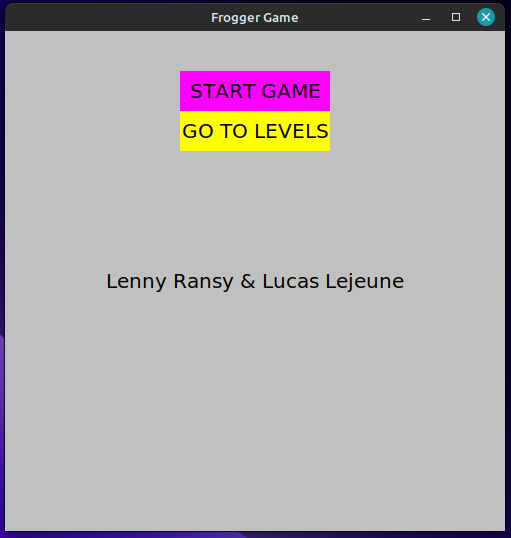
\includegraphics[width=\linewidth]{Images/welcomescreen.png}
      \caption{Menu d'accueil}
    \end{minipage}
    \hfill
    \begin{minipage}{0.3\textwidth}
      \centering
      \vspace{0.35cm}
      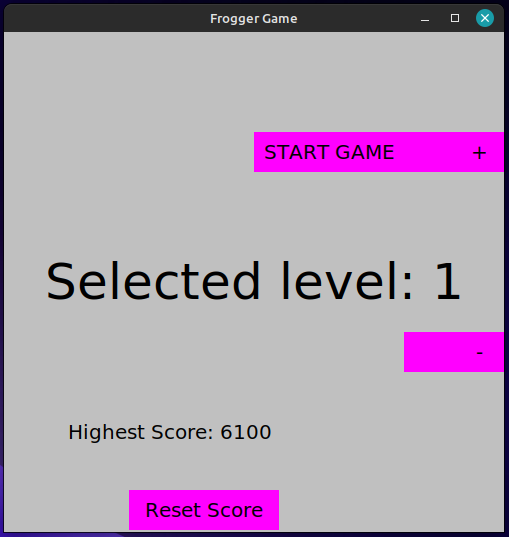
\includegraphics[width=\linewidth]{Images/levelselector.png}
      \caption{Menu de sélection des niveaux}
    \end{minipage}
    \hfill
    \begin{minipage}{0.3\textwidth}
      \centering
      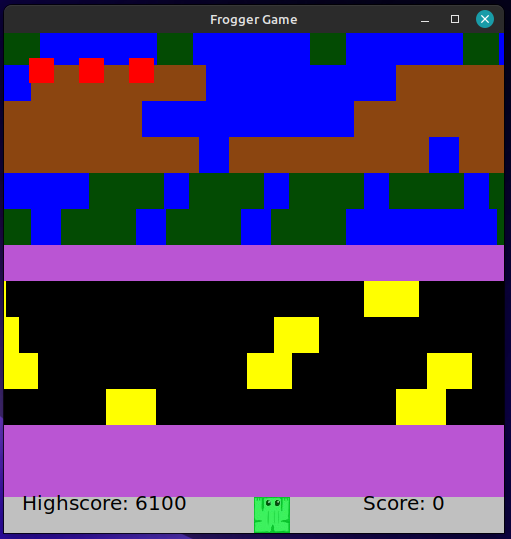
\includegraphics[width=\linewidth]{Images/gamescreenshot.png}
      \caption{Niveau 1}
    \end{minipage}
\end{figure}

\end{document}
